\section{Strategy for Scaling and Updates}\label{sec:scaling}

Our strategy for scaling and updates is based on our choice of deploying the app and the auxilliary services through an container orchestration platform, namely \textit{Docker Swarm}. We chose Docker Swarm specifically because installation of Docker was already a part of our automated provisioning procedure, so it would reuire no extra installations.
As such, we could readily migrate from our initial Docker Compose-setup to Docker Swarm.

Currently, our provisioning script creates four virtual machines for a fresh provisioning of our entire project:

\begin{itemize}
	\item One VM for a a Docker Swarm \textit{manager}-node
	\item Three VM's as Docker Swarm \textit{worker}-nodes
\end{itemize}

The three worker nodes run a replica of the app.
The manager-node runs all the auxilliary services, and provides load balancing to the three worker nodes.
This setup works well, because we want to centralize our logging and monitoring, as they are not under variable load from the public internet: It's only the system owners and administrators that need to access those.
Furthermore, it is trivial to store the logs on the disk of the single manager-node, which is otherwise a challenge in Docker Swarm environments.

However, we have not implemented an automatic scaling strategy. For now, the strategy is to monitor the traffic and manually provision more worker nodes if needed.

\begin{figure}
	\begin{center}
		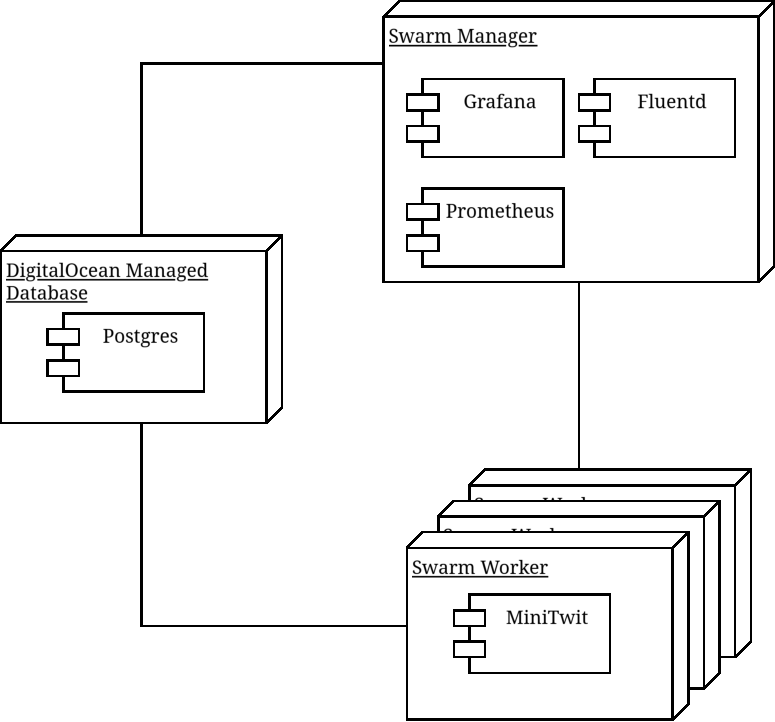
\includegraphics[width=0.50\textwidth]{img/deployment.pdf}
	\end{center}
	\caption{Deployment view of our system.}\label{fig:deployment}
\end{figure}

We have chosen \textit{rolling updates} as our update strategy, since it allows us to add many more worker-nodes, without much consideration for how the updates will perform.
Furthermore, when using Docker Swarm, it is trivial to enable rolling updates: The addtion of the few lines below in the \texttt{deploy}-section of the \textit{Docker Stack} configuraiton achieves it:

\begin{lstlisting}
update_config:
  parallelism: 1
rollback_config:
  parallelism: 1
\end{lstlisting}

Here, we specify that at most one worker-node must be under update. This ensures a maximum peformance under a system update.
Furthermore, we also specifiy that, in the case of failure of a new update, rollbacks should also only be performed on one node at the time
Furthermore, we also specifiy that, in the case of a need to revert a new update, rollbacks should also only be performed on one node at the time.
While both these choices have the consequence of out-of-date versions of the system being online for a non-minimal amount of time, we prioritize system performances over the speed of version changes.







